\documentclass[12pt]{scrbook}

\usepackage[T1]{fontenc}
\usepackage[utf8]{inputenc}
%\usepackage[ngerman]{babel}
\usepackage{mathrsfs}
\usepackage{amsmath, amssymb, amsfonts, amsthm}
\usepackage{array}
\usepackage{cite}
\usepackage{braket}
\usepackage{dsfont}
\usepackage{listings}
\usepackage{graphicx}
\usepackage{color}
\usepackage{framed}
\usepackage{caption}
\usepackage[automark]{scrpage2}
%\usepackage[export]{adjustbox}
\usepackage{verbatim}

\usepackage{float}

\newcommand{\changefont}[3]{\fontfamily{#1}\fontseries{#2}\fontshape{#3}\selectfont}

\usepackage[hyperfigures =true ,linkcolor =black, urlcolor=blue, colorlinks =true, citecolor=black ,pdfauthor ={ Leonard Peter Wossnig},pdftitle ={exercises in HPCSE},pdfcreator ={ pdfLaTeX }]{hyperref}

\definecolor{mygray}{rgb}{0.98,0.98,0.98}
\definecolor{darkgray}{rgb}{0.6,0.6,0.6}
\definecolor{mygreen}{rgb}{0.0,0.5,0.0}
\definecolor{myblue}{rgb}{0.0,0.0,0.5}
%\definecolor{mypurple}{rgb}{0.5,0.0,0.5}

\lstdefinelanguage[]{CodeBlocks}{classoffset=0, language=C++,commentstyle=\tiny\color{darkgray}, comment=[l]{//},morecomment=[s]{/*}{*/}, columns=flexible, basicstyle = \tiny, backgroundcolor=\color{mygray}, frame=single, keepspaces=false, keywordstyle=\color{red}, breaklines = false, aboveskip = 1.2em,belowskip = 1.5em, directivestyle=\color{mygreen}, ,classoffset=2, otherkeywords={(,),[,],<<,>>,++,--,=,+=,-=,;,&,&&,+,-,!,\{,\},::,<,>,\#}, classoffset=0, emph={bool, double, int, for, if, else, ifelse, return, void, namespace, using, const, float, long, }, emphstyle=\color{blue}, stringstyle = \color{darkgray}}



\begin{document}

\section{Exercise 4 - HPCSE - Leonard Wossnig}
\subsection{Task 1.}
The proof is the following:
\begin{align}
E \left[ \frac{N}{N-1} (<X^2> - <X>^2) \right] =  \frac{N}{N-1} E \left[(<X^2> - <X>^2) \right] = \notag \\
\frac{N}{N-1} \left[<X^2> - \frac{1}{N} <X^2> - \frac{N-1}{N} <X^2>\right] = <X^2> - <X>^2 = \text{Var} (X)
\end{align}

\subsection{Task 2.}
The code I build and used behaved quite slow. The timing for the runs was highly time consuming so the question arises if this comes either from the bad implementation of the seeding and RNG initialization or as a result from the algorithm itself. MC methods (especially in this case with random walks) are very time consuming. In the case of this approach we have a two dimensional integral, where also MC seems not a good method to approach. \\
My question is, how could I improve the appended code to decrease runtime?\\

The strong scaling behaviour resulted in the following plot while the errors decrease with the number of runs: \\
\begin{minipage}[!t]{0.5\textwidth}
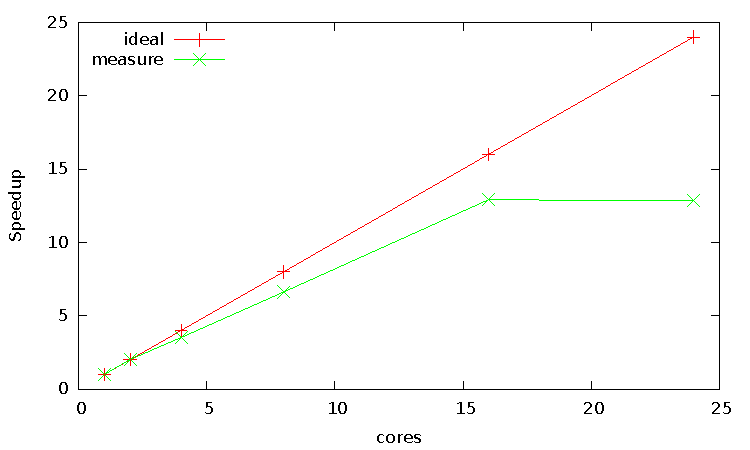
\includegraphics[width=\textwidth, keepaspectratio]{strong_scaling.pdf}
\end{minipage}
\begin{minipage}[!t]{0.5	\textwidth}
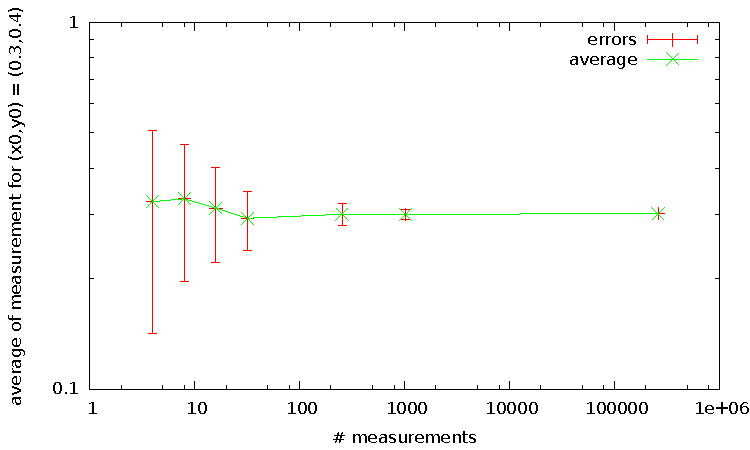
\includegraphics[width=\textwidth]{errors.pdf}
\end{minipage}


\subsection{Appendix}
In the following i append the source code of some of the tasks:\\
\begin{lstlisting}[language=CodeBlocks]
  1 
  2 #include <omp.h>
  3 #include <iostream>
  4 #include <algorithm>
  5 #include <string>
  6 #include <fstream>
  7 #include <vector>
  8 #include <cmath>
  9 #include <random>
 10 #include "timer.cpp"
 11 #define _PARALLEL
 12 //#define _DEBUG
 13 #define pi 3.14159265359
 14 
 15 typedef double value_type;
 16 typedef std::size_t size_type;
 17 
 18 class Diffusion2D {
 19 
 20 /*********************************************************/
 21 /*********************************************************/
 22 public:
 23     Diffusion2D(const value_type D,
 24                 const value_type L)
 25     : D_(D), L_(L)
 26     {}
 27    // D unneccesary here but left in for trial of a D-dependend trial of random walks...
 28 
 29 /*********************************************************/
 30     static value_type rho_function(value_type x, value_type y)
 31     {
 32             return x;
 33     }
 34 
 35 /*********************************************************/
 36     value_type advance(value_type x, value_type y, int Nin)
 37     {
 38 
 39 
 40           const value_type d = 0.01;
 41           int N = Nin;
 42           value_type sum = 0.;
 43 
 44 #ifdef _PARALLEL
 45           #pragma omp parallel for reduction(+:sum)
 46 #endif
 47           for( size_type k=0; k<N ; k++ )
 48           {
 49                   value_type delta_x = x, delta_y = y;
 50                   std::random_device rd;
 51                   std::mt19937 mt2(rd());
 52                   std::uniform_real_distribution<value_type> ureal_d(0.,1.);
 53                   // iteration random walk till border crossed
 54 #ifdef _DEBUG
 55 #pragma omp critical (output)
 56                   std::cout << "Thread " << omp_get_thread_num() << " going into while loop" << std::endl;
 57 #endif
 58                   while(true)
 59                   {
 60                           delta_x += d*std::cos(2 * pi * ureal_d(mt2) );
 61                           delta_y += d*std::sin(2 * pi * ureal_d(mt2) );
 62                           if( (delta_x >= L_) || (delta_y >= L_) || (delta_x <= 0.) || (delta_y <= 0.) )
 63                           {
 64                                   break;
 65                           }
 66                   }
 67 
 68                   // if border crossed --> add rho(x_c,y_c) to sum
 69                   // incase i want to adjust the exact position determination i can adjust different for crossing of x and y boder
 70                   // but in this case it should average equally if i just take the position at the end of the crossing step
 71                   if( (delta_x >= L_/2.) || (delta_y >= L_/2.) || (delta_y <= 0.) )
 72                   {
 73                           sum += rho_function(delta_x, delta_y) ;
 74                   }
 75                   else//if( (delta_x <= 0.) || (delta_y <= 0.) )
 76                   {
 77                           sum += 0;
 78                   }
 79           }
 80           return (sum/N);
 81     }
 82 
 83 
 84 /*********************************************************/
 85 
 86     void write_density(value_type sum, std::string const& filename) const
 87     {
 88         std::ofstream out_file(filename, std::ios::out);
 89         out_file << sum << std::endl;
 90         out_file.close();
 91     }
 92 
 93 
 94 /*********************************************************/
 95 /*********************************************************/
 96 
 97 private:
 98     value_type D_, L_;
 99 /*********************************************************/
100 };
101 
102 
103 int main(int argc, char* argv[])
104 {
105     if (argc < 4) {
106         std::cerr << "Usage: " << argv[0] << " D L N" << std::endl;
107         return 1;
108     }
109 
110     const value_type D  = std::stod(argv[1]);
111     const value_type L  = std::stod(argv[2]);
112     int              Nin  = std::stod(argv[3]);
113 
114 
115 
116     Diffusion2D system(D, L);
117     value_type sum;
118     Timer t;
119 
120     t.start();
121     sum = system.advance(0.3,0.4, Nin);
122     system.write_density(sum ,"density_0.3_0.4.dat");
123     t.stop();
124 
125     //std::cout << "Timing : " << t.duration() << std::endl;
126     std::cout << sum << std::endl;
127 
128     return 0;
129 }
\end{lstlisting}

while for multiple runs the program was executed with the following script file:
\begin{lstlisting}[language=CodeBlocks]
  1 #!/bin/bash
  2 for ((i = 1; i <= 100; i++))
  3 do
  4         ./diffusion2d_serial.exe 1 1 1024 >> average_rho_1024.txt
  5         echo "run $i"
  6 done
\end{lstlisting}
\end{document}